\chapter{Μηχανισμός δημοπρασίας}
\InitialCharacter{Ο} μηχανισμός δημοπρασίας λειτουργεί ως βασικό συστατικό της προτεινόμενης αποκεντρωμένης εφαρμογής (\en{dApp}), δημιουργώντας μια διαφανή και δίκαιη πλατφόρμα για την κατανομή των υπολογιστικών εργασιών. Η παρούσα ενότητα διευκρινίζει την περίπλοκη δυναμική της διαδικασίας δημοπρασίας, τις στρατηγικές υποβολής προσφορών που χρησιμοποιούν οι πάροχοι και τα κριτήρια που καθοδηγούν την επιλογή ενός παρόχου από έναν πελάτη.

\section{Επισκόπηση της διαδικασίας δημοπρασίας}
Η διαδικασία δημοπρασίας ξεκινά όταν ένας πελάτης υποβάλλει μια υπολογιστική εργασία στην \en{dApp}. Η διαδικασία αυτή είναι δομημένη ώστε να διασφαλίζεται η δικαιοσύνη, η διαφάνεια και η βέλτιστη κατανομή εργασιών:
\begin{enumerate}
    \item Υποβολή εργασίας: Οι πελάτες ξεκινούν τη δημοπρασία αναφέροντας τις λεπτομέρειες της υπολογιστικής εργασίας και συγκεκριμένα την αναμενόμενη προθεσμία ολοκλήρωσης και τη σχετική συμβολοσειρά επαλήθευσης.
    \item Υποβολή προσφορών: Μετά την υποβολή της εργασίας, οι πάροχοι έχουν την ευκαιρία να εξετάσουν τις λεπτομέρειες της εργασίας και να υποβάλλουν προσφορές με την προτεινόμενη τιμή τους (σε \en{wei} ανά δευτερόλεπτο εκτέλεσης της εργασίας).
    \item Επιλογή παρόχου: Όσο η δημοπρασία παραμένει ενεργή, ο πελάτης μπορεί να επιλέξει τον πάροχο που επιθυμεί, βασιζόμενος σε διάφορους παράγοντες που θα αναλυθούν παρακάτω. Η απόφαση αυτή σηματοδοτεί την ολοκλήρωση της δημοπρασίας και την έναρξη της φάσης εκτέλεσης της εργασίας.
\end{enumerate}

Παρακάτω παρουσιάζεται ο κύκλος ζωής μιας δημοπρασίας, με βάση την κατάσταση \en{AuctionState} της οντότητας \en{Auction}.
\begin{illustration}
    \centering
    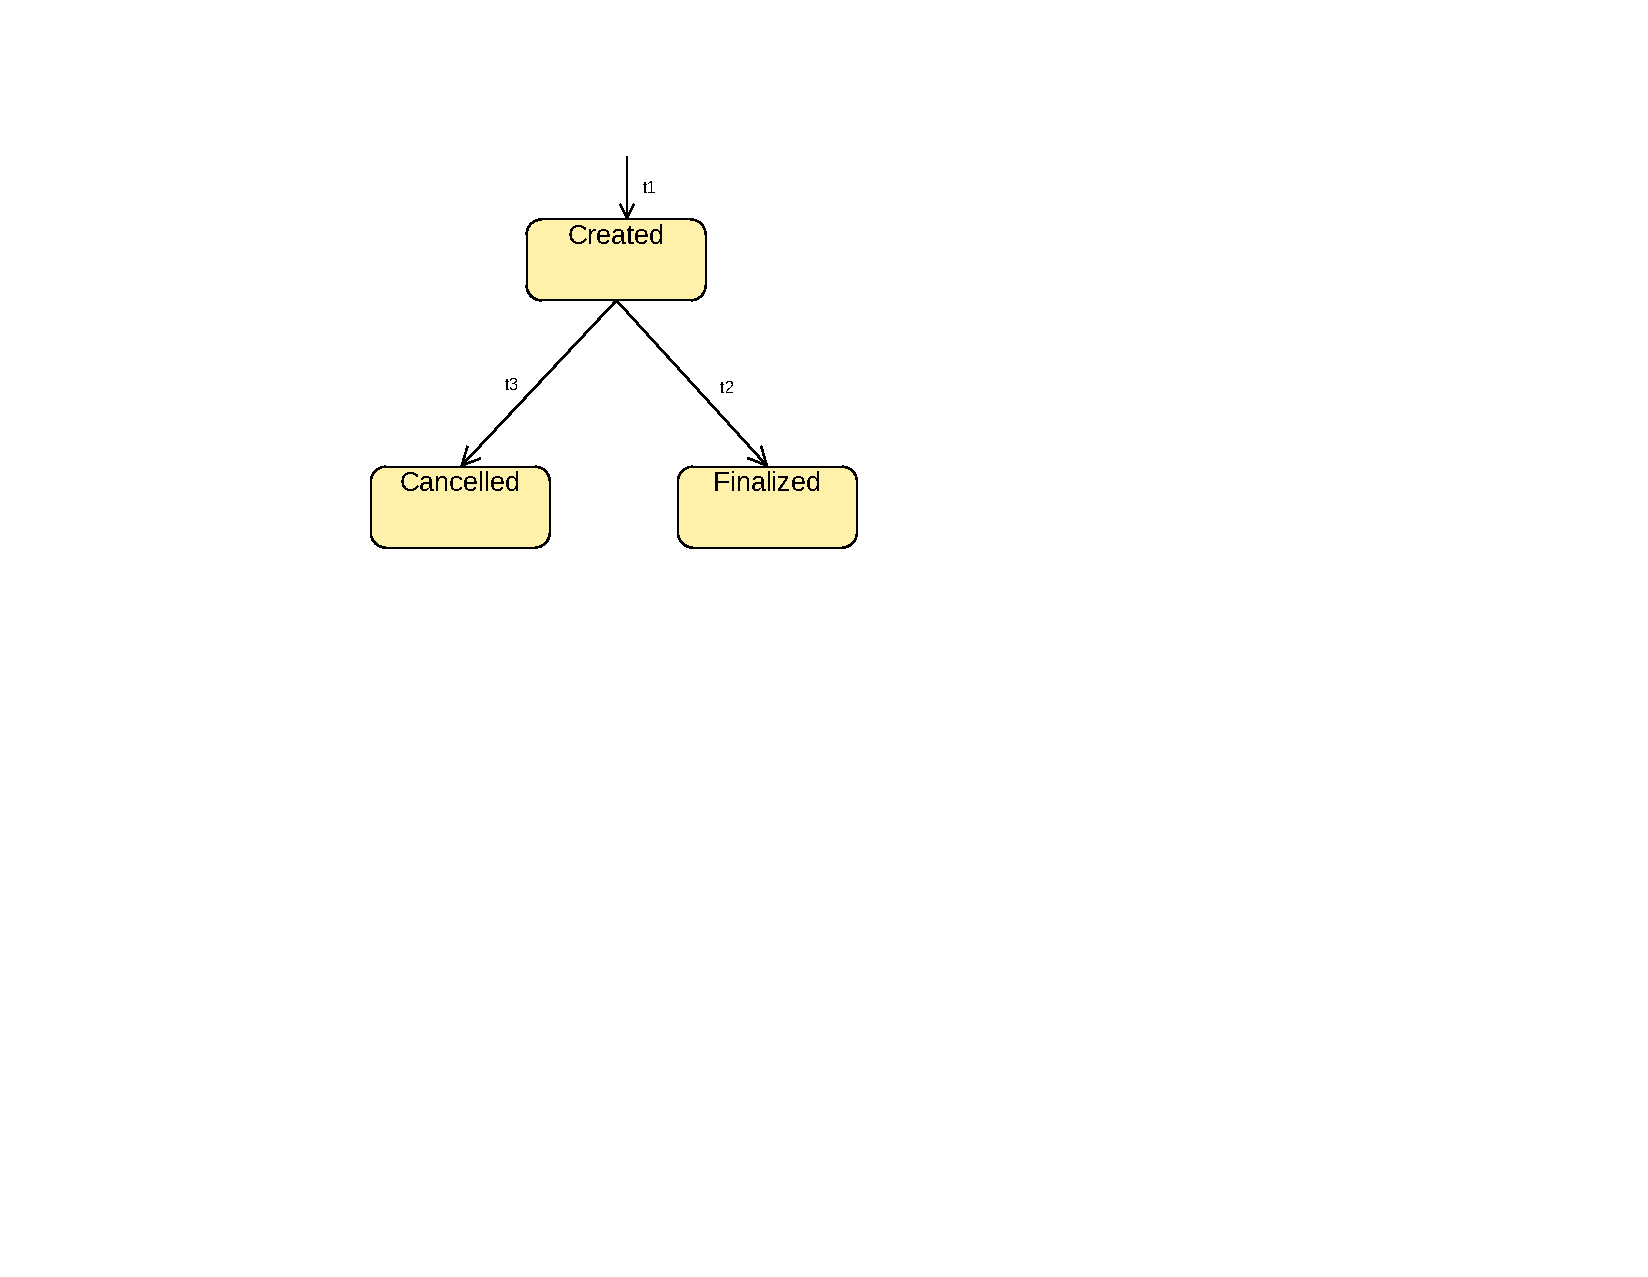
\includegraphics[width=0.8\textwidth]{figures/figure-006.pdf}
    \caption{\en{State machine} του \en{Auction}, με βάση το \en{AuctionState}} 
    \begin{minipage}{\textwidth}
        \centering
        \small
        \text{Οι μεταβάσεις \en{t1, t2} και \en{t3} πραγματοποιούνται από τον \en{client}}.
      \end{minipage}
\end{illustration}

\newpage

\section{Μηχανισμός βαθμολόγησης}
Στο \en{smart contract} \en{TasksManager} αποθηκεύεται το ιστορικό των επιδόσεων των παρόχων και των πελατών στην διαδικασία μέσω ενός μηχανισμού βαθμολόγησης. Ο μηχανισμός αυτός είναι καθοριστικής σημασίας για τη διατήρηση της ακεραιότητας της \en{dApp}, διασφαλίζοντας ότι τόσο οι πάροχοι όσο και οι πελάτες λογοδοτούν για τις πράξεις και τις επιδόσεις τους.
\begin{itemize}
    \item Βαθμολογία του παρόχου: Σε κάθε πάροχο αποδίδεται μια βαθμολογία, η οποία προκύπτει από τον συνδυασμό των ανεπιτυχών (\en{downVotes}) και επιτυχών (\en{upVotes}) εκτελέσεων εργασιών, η οποία αντικατοπτρίζει το ιστορικό των επιδόσεων τους. Ο υπολογισμός της βαθμολογίας χρησιμοποιεί τη μεθοδολογία 'ταξινόμησης εμπιστοσύνης' που βασίζεται στο διάστημα βαθμολογίας \en{Wilson}, έναν διάσημο αλγόριθμο που χρησιμοποιείται από πλατφόρμες όπως το \en{Reddit} για την ταξινόμηση των σχολίων στην πλατφόρμα \cite{ref49}. Με τον τρόπο αυτό διασφαλίζεται ότι η βαθμολογία δεν είναι απλώς ένας μέσος όρος, αλλά μια αναπαράσταση της αξιοπιστίας του παρόχου με βάση τον όγκο και την αναλογία των \en{upvotes} προς τα \en{downvotes} του. 
    \item Βαθμολογία πελάτη: Στους πελάτες αποδίδεται επίσης μια αντίστοιχη βαθμολογία, ενδεικτική των ιστορικών αλληλεπιδράσεών τους και της συνέπειάς τους στην αμοιβή των παρόχων για επιτυχώς εκτελεσμένες εργασίες. Η βαθμολογία αυτή παίζει καθοριστικό ρόλο στη διαμόρφωση της στρατηγικής προσφορών του παρόχου.
\end{itemize}

\section{Κριτήρια που καθοδηγούν τον πελάτη στην επιλογή παρόχου}
Η επιλογή του παρόχου από τον πελάτη επηρεάζεται από μια σειρά παραγόντων, διασφαλίζοντας ότι η απόφαση είναι τόσο τεκμηριωμένη όσο και βέλτιστη:
\begin{itemize}
    \item Προσφορά τιμής: Η προτεινόμενη τιμή του παρόχου παραμένει πρωταρχικής σημασίας, με τους πελάτες να κλίνουν φυσικά προς τις ανταγωνιστικές τιμές.
    \item Το ιστορικό επιδόσεων του παρόχου: Η βαθμολογία του παρόχου, όπως υπολογίζεται με την προαναφερθείσα μεθοδολογία, προσφέρει πληροφορίες σχετικά με την αξιοπιστία και τις προηγούμενες επιδόσεις του.
    \item Προηγούμενες συνεργασίες: Προηγούμενες συνεργασίες με τον συγκεκριμένο πάροχο που κατέληξαν σε θετικά αποτελέσματα μπορούν να επηρεάσουν σημαντικά την απόφαση ενός πελάτη.
\end{itemize}

\section{Παράγοντες που διαμορφώνουν τη στρατηγική προσφορών του παρόχου}
Οι πάροχοι, κατά τη διαμόρφωση των προσφορών τους, εξετάζουν πληθώρα παραγόντων για να βελτιστοποιήσουν τις πιθανότητές τους να επιλεγούν, εξασφαλίζοντας παράλληλα την κερδοφορία τους:
\begin{itemize}
    \item Η αξιοπιστία του πελάτη: Η βαθμολογία ενός πελάτη, ενδεικτική των προηγούμενων αλληλεπιδράσεών του και της συνέπειας των πληρωμών του, μπορεί να επηρεάσει το ποσό της προσφοράς του παρόχου.
    \item Διαθεσιμότητα πόρων του παρόχου: Οι πάροχοι με άφθονους πόρους ενδέχεται να έχουν την προδιάθεση να υποβάλουν χαμηλότερη προσφορά για να εξασφαλίσουν την εργασία.
    \item Ιστορικό αλληλεπιδράσεων με τον πελάτη: Οι θετικές αλληλεπιδράσεις του παρελθόντος με τον πελάτη μπορούν να παρακινήσουν έναν πάροχο να υποβάλει μια πιο ανταγωνιστική προσφορά.
\end{itemize}

Συνοψίζοντας, ο μηχανισμός δημοπρασίας, ο οποίος υποστηρίζεται από τη διαφανή διαδικασία υποβολής προσφορών, τα κριτήρια αξιολόγησης και το σύστημα βαθμολόγησης, ενισχύει τη δέσμευση της \en{dApp} για την προώθηση ενός αξιόπιστου και αποτελεσματικού περιβάλλοντος για την αποκεντρωμένη εφαρμογή υπολογιστικής νέφους.
